\section{Introduction}\label{sec:Intro}
Although peak (or valley) current mode control (PCC) has been widely used in dc-dc voltage regulator control for a long time, high frequency \footnote{switching frequency $> 1$ MHz} dc-dc converters using PCC are seldomly reported in the literature.

Parasitic ringing is an important bottleneck when implementing PCC for high-frequency dc-dc converters. The severe voltage spikes are common in a high frequency power converts using PCC as shown in \ref{fig:noisecurrent}. In one of our experiments, when these harsh parasitic ringings contaminate current measurements, the inner current loop of a current-mode buck converters using constant on-time (CM-COT) buck converter can actually be unstable. This phenomena challenges the traditional understanding that in CM-COT buck converters, {\color{red} the inner current loop} is deadbeat and stable at all operating points \cite{Redl1981}. In this paper, we provide new theoretical criteria which explain why and predict when this instability phenomena happen.
% We also prove that the stability margin can be improved by slowing down the controller bandwidth.

It is impossible to decrease the parasitic inductance under the level of $n$H under the constraints of the current pc board technology. Therefore, we solve this problem in another way: instead of eliminating parasitic ringings, we show three new compensation techniques which guarantee the PCC to work in harsh parasitic ringing conditions - analog comparator overdrive propagation delay {\color{red}(COPD)}, slope compensation and low-pass filter. We show that the overdrive propagation delay of the analog comparator can be eliminate the effect of parasitic ringing interference on the plant. We explain that the slope compensation, which is widely used in fixed-frequency PCC, can also be used in variable-frequency PCC to reject the parasitic ringing interference. We claim that a low-pass filter with cut-off frequency slower than switching frequency can still result in a good performance.
Furthermore, unlike the traditional compensation design methods based on rule-of-thumbs and design experiences, we show a rigorous analysis tool to help designer with the design procedure.

PCC is advantageous in high-frequency and fast-transient-response dc-dc converters over the other traditional control methods including voltage-mode control and ripple-based control. Peak current mode control shows significantly faster transient response and is much easier to design than the voltage mode control \cite{erikson2007}. Power converter plant in PCC architecture is usually a lower order system compared to voltage mode control because the PCC architecture eliminates the transient from duty cycle to inductor current by measuring and commanding inductor current \cite{Bram2015tpel}. A low order plant makes the compensator design easier and more robust. Peak current mode control is more robust to the output capacitor parasitic and can be applied in any types of dc-dc converters compared to the ripple-based method \cite{Redljian2009tpel}. PCC sense and control the inductor current directly while the ripple-based control has to rely on the assumption that the capacitor voltage contains the information of inductor current. PCC does not rely on the output capacitor and load information, but the ripple-based method can even go in instability if the ESR or ESL is not appropriate. PCC can fix the switching frequency more easily but ripple based control suffers a lot from the jittering in switching frequency. PCC can provide a tight DC voltage regulation. Another important benefit is that PCC naturally does cycle-by-cycle over current protection to the power stage, hence the fault protection design can be simplified. 

Among many PCC architectures in literature, direct PCC using the mixed-signal hardware implementation is one of the most popular approach because it has both fast transient response and programmable flexibility. By whether the inductor current is sensed or not, state-of-the-art PCC can be direct PCC methods and indirect methods. Among direct PCC methods, mixed-signal implementation is the most promising because it shares the benefits of fast transient response and ability to be quickly online tuned to adapt to fast varying operating points. Analog implementation is the most traditional implementation method: The output voltage is processed by an error amplifier and the result is compared with the sensed current signal by an analog comparator \cite{Kaz2006tcs}. Although the design methods are well-established and it is not hard to obtain high control bandwidth, good dynamic performance is not always guaranteed in a wide operating voltage range because {\color{red} electrical dynamics} of circuits change with output voltage operating points and load conditions \cite{erikson2007}. Digital implementation guarantees the programmable flexibility of the adaptive voltage regulation: An analog-to-digital converter (ADC) is added to discretize the sampled inductor current. Then the quantified current is compared with the current command in through digital logic. The implementation of the inductor current sampling can be referred to \cite{Lilee2008APEC}. It is not suitable for high-frequency converter because a high-speed sampler is required. Mixed-signal hardware implementation \cite{Prodic2011tcs} \cite{Huerta2012} combines the advantages of both analog and digital implementations. A common mixed-signal structure includes a digital voltage control loop and an analog current loop.

Because of the difficulties in measuring inductor current in high-frequency power converters, several indirect PCC are proposed. However, currently proposed indirect PCC  still cannot outperform the direct PCC.
Current-programmed control constructs the inductor current waveform using the priori-model and control the inductor current indirectly by duty ratio.
The classic current-programmed control \cite{Chendragan2003} is sensitive to the time-varying uncertainties of the inductor model and the input/output voltage measurement. Although \cite{Taeed2014} improves the method by measuring the actual current at two points every cycle and calculate slope, the prediction error is still inevitable because in some applications where the inductor current can go highly non-linear \cite{Ahsanuzzamanprodic2012apec} \cite{DiCapua2016}. Hence curve fitting using 2 sample points can cause significant errors. Another method in \cite{Chattopadhyay2006} claim a control algorithm which is stable under the incorrect current ramp estimation, but the proposed method cannot guarantee fast transient response.
A V\textsuperscript{2}I\textsubscript{c} method by \cite{Huerta2013} measures and control the capacitor current which contains the inductor current information.
However, a complicated impedance matching network has to be designed to compensate the output capacitor parasitic 
\cite{Huerta2009a}. Several derivative output ripple voltage (DORV) techniques get the capacitor current information by differentiating the capacitor voltage \cite{Mai2008} \cite{Chen2017}. Although the methods avoid the complicated capacitor current measurement, it is vulnerable to noises because of derivative calculation. 
Several papers combine the aforementioned current mode control techniques with other control methods, for example, \cite{Huang2002} combines the peak current mode control and the ripple-based control. \cite{Cheng2014a} is the digital version of \cite{Huang2002}. \cite{Cheng2013} and \cite{Liu2018} combines ripple-based control with the current-programmed control and derivative output ripple voltage technique respectively. There also exist a few current-mode control methods which is not within the aforementioned category, for example, \cite{Kurokawa2016} uses the inductor current feed-forward in voltage mode control. \cite{Saggini2004} Implements a current-programmed control with an synchronously sampled output voltage.

Main factors which restrict the control bandwidth of dc-dc converters using PCC are low-loss switching devices, high-speed digital control devices and low circuit parasitics. Recently, the commercial GaN FET already has low enough switching losses which enables the high frequency DC-DC converter using hard switching \cite{Huang2014c}.
People can get access to high speed digital control device. For example, a commercial ADC with precision over 10 bits can have sampling latency lower than 50\,ns \cite{dsAD9215,dsMAX1214}, In the market, there are several types of DAC with settling time lower than 20\,ns \cite{dsLTC1666, dsAD9744} and FPGA with main clock higher than 400\,MHz \cite{dsARTIX72018}. 

Circuit parasitic is more important in implementing direct PCC because the parasitic ringing causes the current measurement and current command error. However, the frequency and time constant of ringing are limited by the minimal parasitic inductance on PCB technology which is in the level of nH. The induced voltage spike is comparable to the voltage on the measurement resistor. Among a few existing works which tackles the high frequency PCC converters problem, either the power level or the power efficiency is sacrificed. Some paper decrease the power rating to avoid ringing interference, but this limited the application area. \cite{Huerta2012} shows a 5MHz converter on board with output power lower than 5\,W. Some use integrated circuit to eliminate the parasitic, but this limit the power level of the circuit. \cite{Trescases2011} reports a 3MHz PCC buck converter on IC. Another method is introducing extra power losses to improve the signal to noise ratio. For example, using damper or snubber to attenuate the energy as well as the amplitude of the ringing. Increasing the sensing resistor value to get a much cleaner current ramp. However, considering the conduction loss is proportional to the square root of current $P_{\text{loss}} = I^2R$ but the signal-to-noise ratio is proportional to the current $V = IR$, this method does more harm than good in large output current applications like voltage regulator modules(VRMs). 

In this paper, instead of trying to eliminate the parasitic ringing, we use several compensation techniques to stabilize the PCC high-frequency power converters even in harsh parasitic ringing conditions. We first exhibit a novel model on the mechanism of how ringing influences the power converter plant and control. Based on the model, we show the rigorous analysis tool to study stability and performance of practical DC-DC converter using PCC. Several compensation techniques are compared and discussed under the analysis tools.

\begin{figure}
\begin{minipage}{0.32\textwidth}
    \centering
    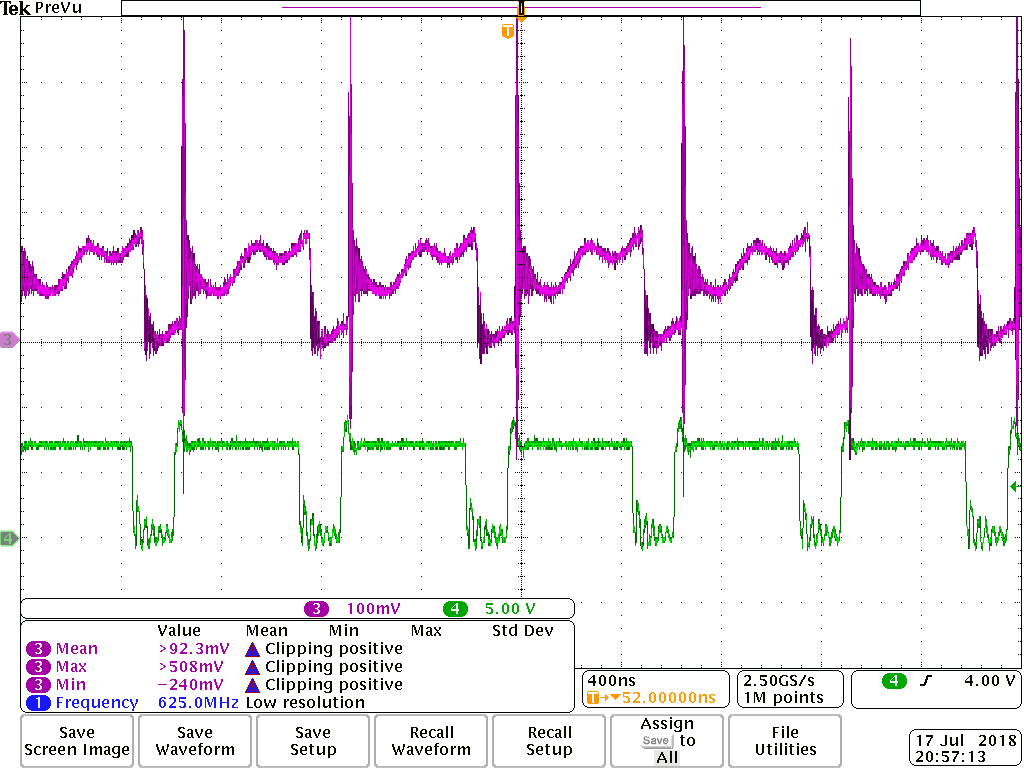
\includegraphics[width=\textwidth]{Figure/section1/ripplecurrent.png}
    \caption{ \label{fig:noisecurrent} Measured inductor current of a digitally-controlled CM-COT boost converter.}
\end{minipage}
%~
% \begin{minipage}{0.32\textwidth}
%     \centering
%     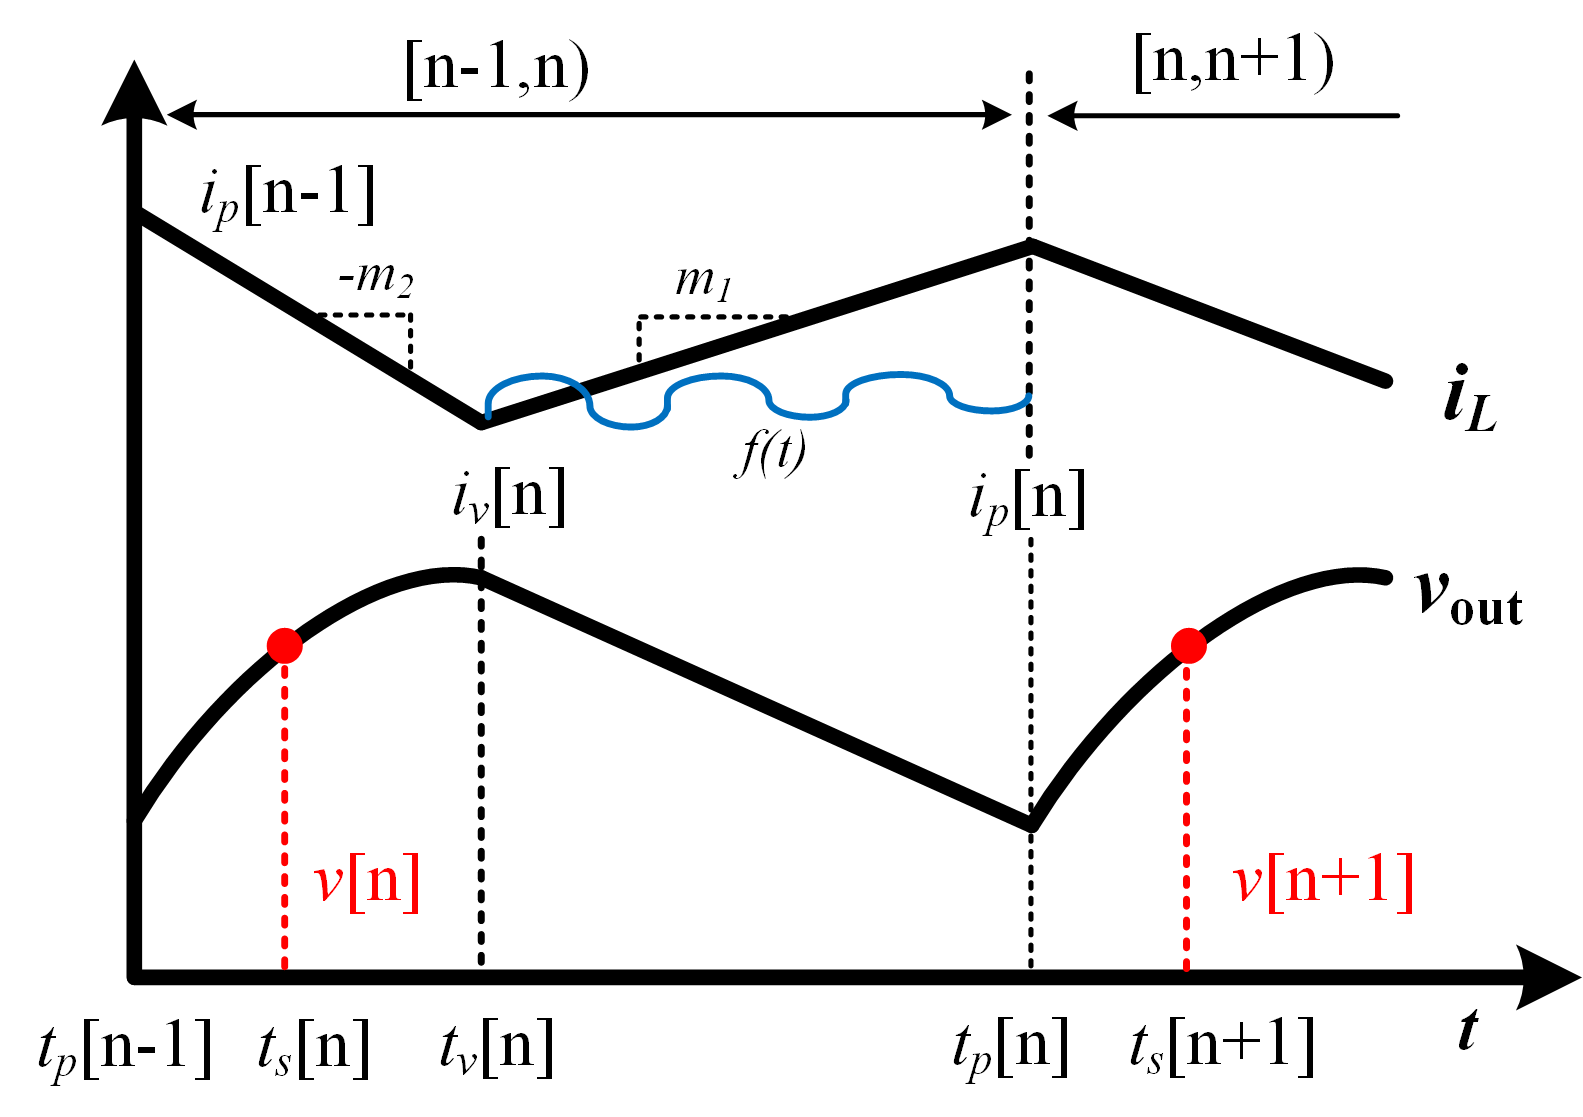
\includegraphics[width=\textwidth]{Figure/section2/eboostwaveform.png}
%   \caption{\label{fig:lcwavefrom} Inductor current and capacitor voltage waveforms of a digitally-controlled CM-COT boost converter.}
% \end{minipage}
~
% \begin{minipage}{0.32\textwidth}
%     \centering
%     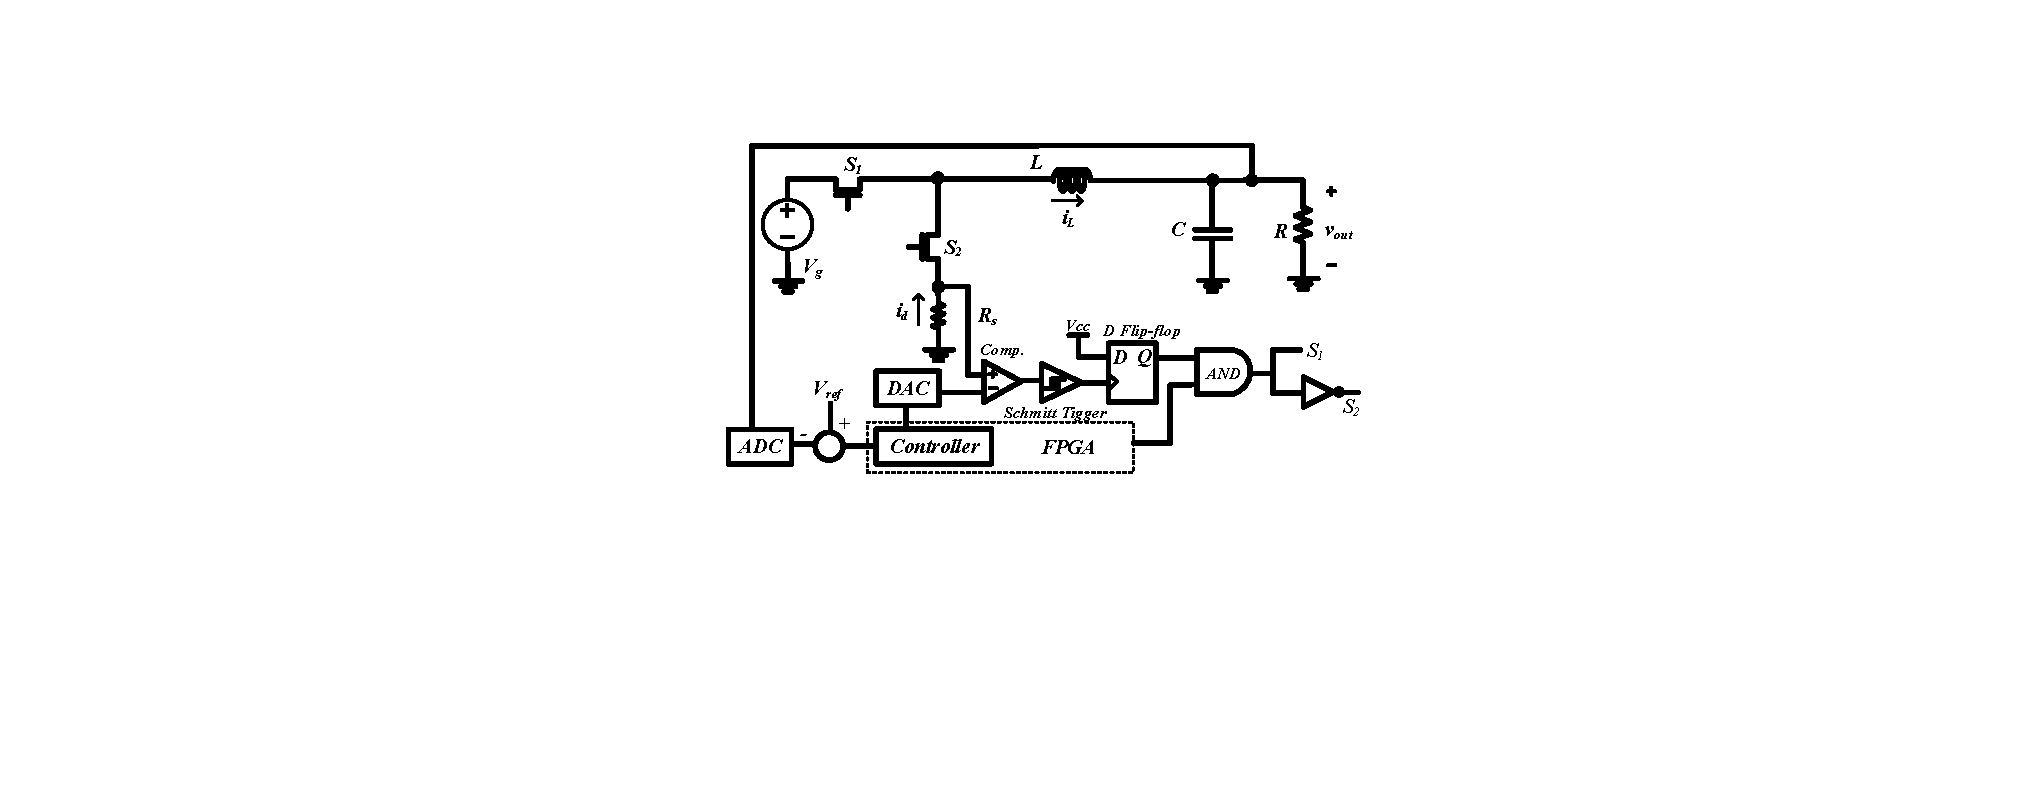
\includegraphics[width=\textwidth]{Figure/section2/currentdetection.pdf}
%     \caption{\label{fig:currentdection} Analog valley-current controller for constant-on-time
%     current-mode buck.}
% \end{minipage}
\end{figure}

